
Details of the MC based background estimations are described below.
Any additional normalizations or uncertainties are summarized
in Table~\ref{tab:mcnorm}.

\begin{table}[htp]
\centering
    \begin{tabular}{|c|cc|}
    \hline
    Background & Normalization Factor & Unceratinty \\ 
    \hline\hline
    $WZ$ & 1.08 & 10~\% \\
    $ZZ$ & 1.05 & 15~\% \\
    %$Z\gamma$ & & 30~\% \\
    $\ttbar +V$ & 1.0 & 30~\% \\
    $ZWW+ZZZ$ & 1.0 & 50~\% \\
    \hline
  \end{tabular}
  

\caption{Summary of normalizations and their uncertainties for the
MC based background estimates used in the analysis.}
\label{tab:mcnorm}
\end{table}



\subsubsection{$WZ\rightarrow lll\nu$}
\label{sec:wzbg}

The $WZ\rightarrow lll \nu$ background is the most important prompt background 
to the $WWW$ signal process. Thus, it must be studied carefully.
The most recent measurements of the $WZ$ process at the LHC
\cite{Aad:2012twa,Anger:1663539,CMS-PAS-SMP-12-006} 
show some tension with the current NLO MC predictions for this process, 
with differences of about 10 to 15\%. 
Studies of other di-boson processes 
\cite{Grazzini:2015nwa,Cascioli:2014yka}
suggest that this could be resolved by 
moving to a NNLO calculation.
For the $WZ$ process, however, this type of calculation is not yet available.
As a result, we instead use the so-called ``2D Sideband'' method
\cite{Aad:2013izg} to derive a correction using the data itself.
This correction is applied to the $WZ$ background MC estimate using
\powheg~mentioned in \sec\ref{sec:www_bg_samples}.

The 2D sideband method is able to determine an estimate
for the process of interest using the data while also correcting
for background contamination. 
To do this, first a signal region 
is chosen which is enriched in the process of interest.
This signal region should have at least two 
independent selection requirements which when inverted suppress
the signal and enhance the backgrounds to that signal.
Next, by inverting one, the other, or both selection requirements, 
three different control regions can be formed
where the signal is suppressed and the backgrounds are enhanced 
with respect to the signal region. 
These control regions are referred to as ``sidebands''.
Furthermore, the three sidebands and the signal region may
related to each other assuming independence of the two different selection
requirements such that the relative change in the backgrounds is the same
when inverting one cut while keeping the other fixed, and vice-versa.
In so doing, one may solve algebraically for the background contamination 
in the signal region and subtract it out, resulting in a pure
estimate of the signal from the data. 


In this case, the signal region is chosen to be enhanced in the $WZ$ process.
The backgrounds to this process are from electroweak contributions (like
$ZZ$, \ttV, and $VVV$) and from backgrounds with fake leptons.
The contributions to the signal region are thus parameterized as
\begin{equation}
\label{eq:wzparam}
N^{\textrm{Data}} =  N^{WZ} + N^{\textrm{Fake}} + N^{\textrm{Electroweak}}
\end{equation}
These backgrounds include processes without \z-bosons.
Thus, the presence of the \z-boson in the signal means that applying a \z-veto of 
$|m_{\textrm{SFOS}}-m_{\z}|<15\GeV$
will remove these contributions to the background.
Also, requiring that the leptons be isolated does a good job of 
removing the fake background.
Thus, the same track and calorimeter isolation requirements
are applied to electrons as muons as in the $WWW$ signal regions
described in \sec\ref{sec:object_selection}.

The \z-veto and the isolation requirements are 
independently inverted\footnote{The thresholds are also slightly shifted 
so that there is a ``dead'' region between the signal regions and sidebands 
which is not used by either. This ensures separation between all regions.}
to form the three sidebands.
The distribution of $m_{\textrm{SFOS}}$ is shown in
\fig\ref{fig:wz_sidebands} in both the the isolated and non-isolated regions.
The expectation in each sideband can be parameterized
in the same way as \eqn\eqref{eq:wzparam}, resulting in one
equation for each region.
One more equation can be found by assuming that the effect of 
the isolation cut on the fake background is independent of the \z-veto.
That is to say, it is assumed that:
\begin{equation}
\label{eq:wz_constraint}
R^{\textrm{Fake}}_{\textrm{With \z-veto}} = R^{\textrm{Fake}}_{\textrm{Without \z-veto}}
\end{equation}
where 
\begin{equation}
R^{\textrm{Fake}}_{A} = 
\frac{N^{\textrm{Fake}}_{A,\textrm{Isolated}}}
{N^{\textrm{Fake}}_{A,\textrm{Non-Isolated}}}
\end{equation}
and where $N^{Fake}_{A,B}$ is the number of fake background
events under conditions $A$ and $B$.
Using this notation we can rewrite \eqn\eqref{eq:wzparam} as:
\begin{equation}
\label{eq:wzparam2}
N^{\textrm{Data}}_{A,B} =  N^{WZ}_{A,B} + N^{\textrm{Fake}}_{A,B} + N^{\textrm{Electroweak}}_{A,B}
\end{equation}
This results in five equations: the expectation,
\eqn\eqref{eq:wzparam2}, from varying the conditions $A$ and $B$ independently,
and \eqn\eqref{eq:wz_constraint}.



\begin{figure}[htp]
\centering
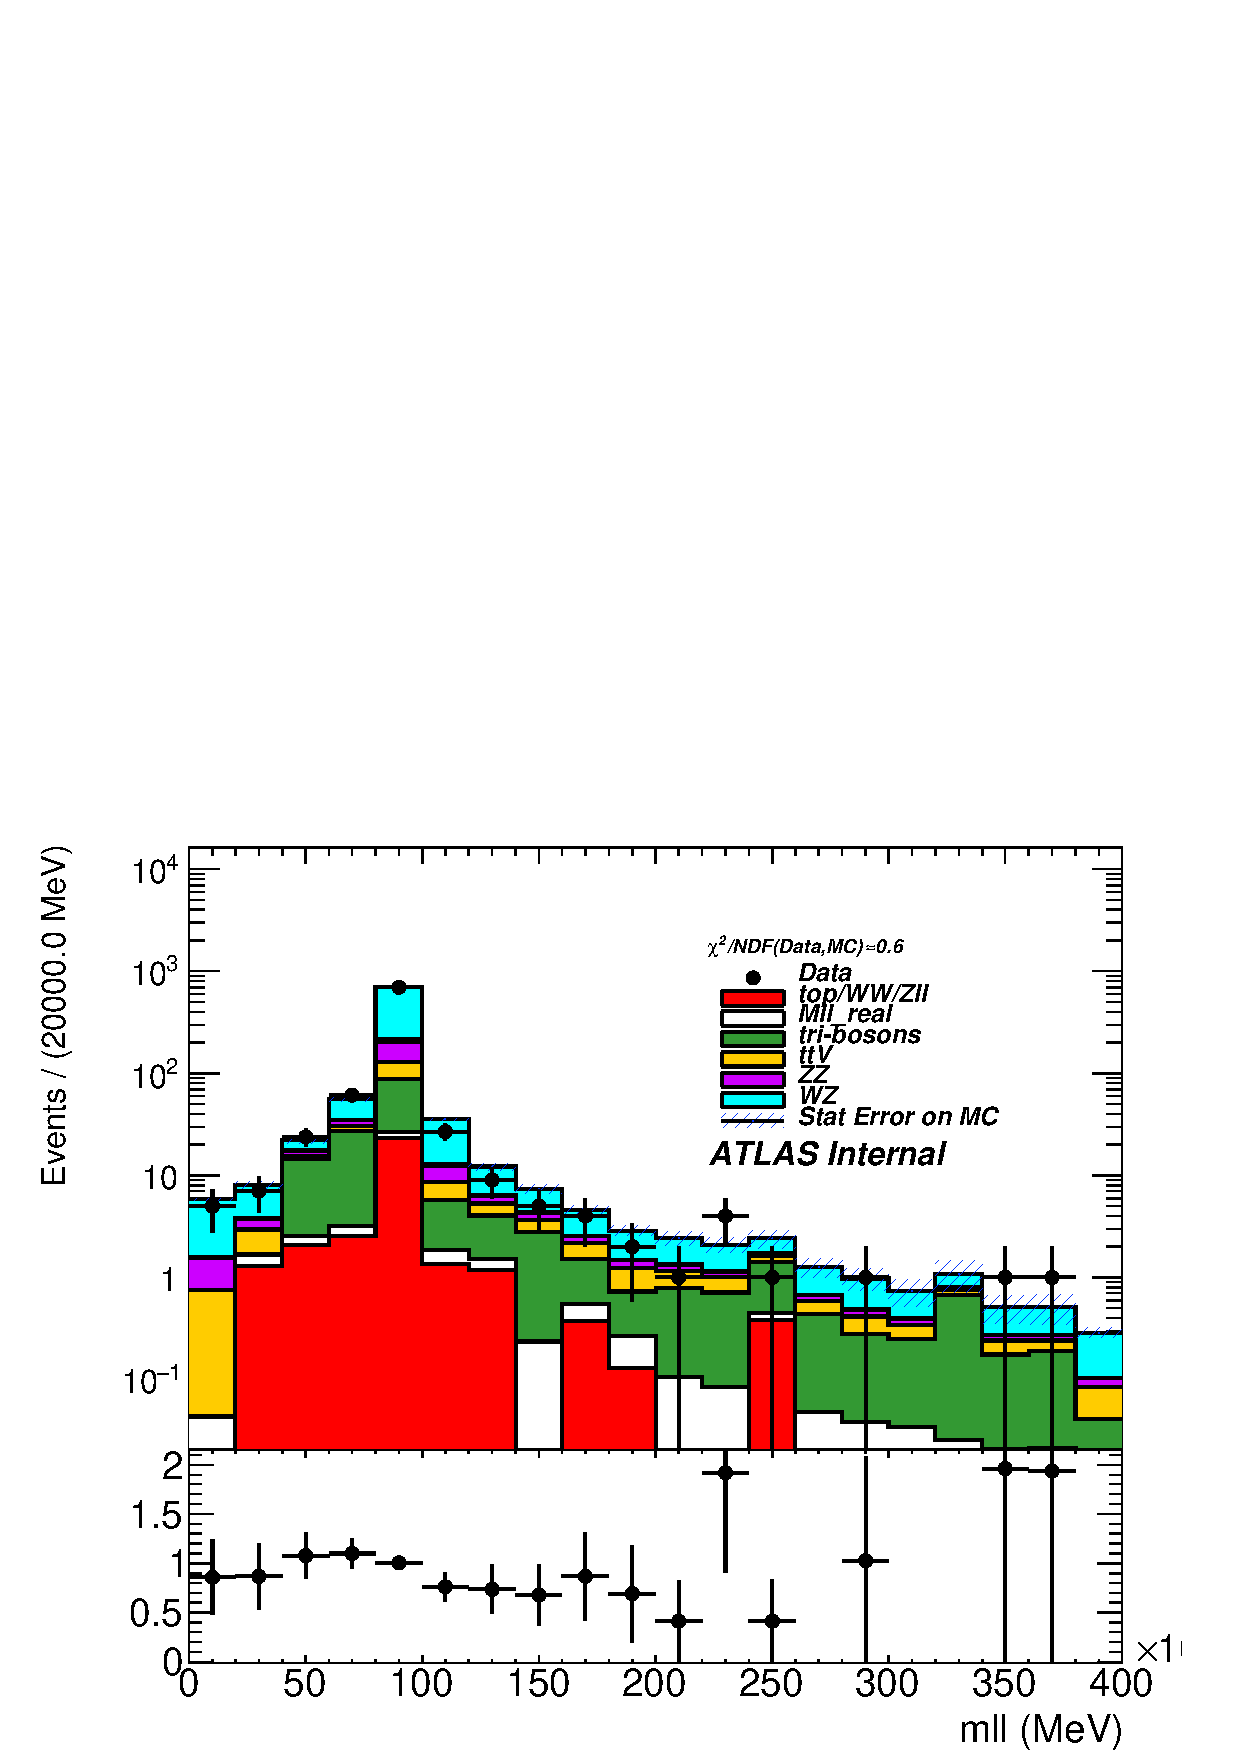
\includegraphics[width=0.45\textwidth]{figures/WZ_CR/2DSideband_WZCR_Isolated}
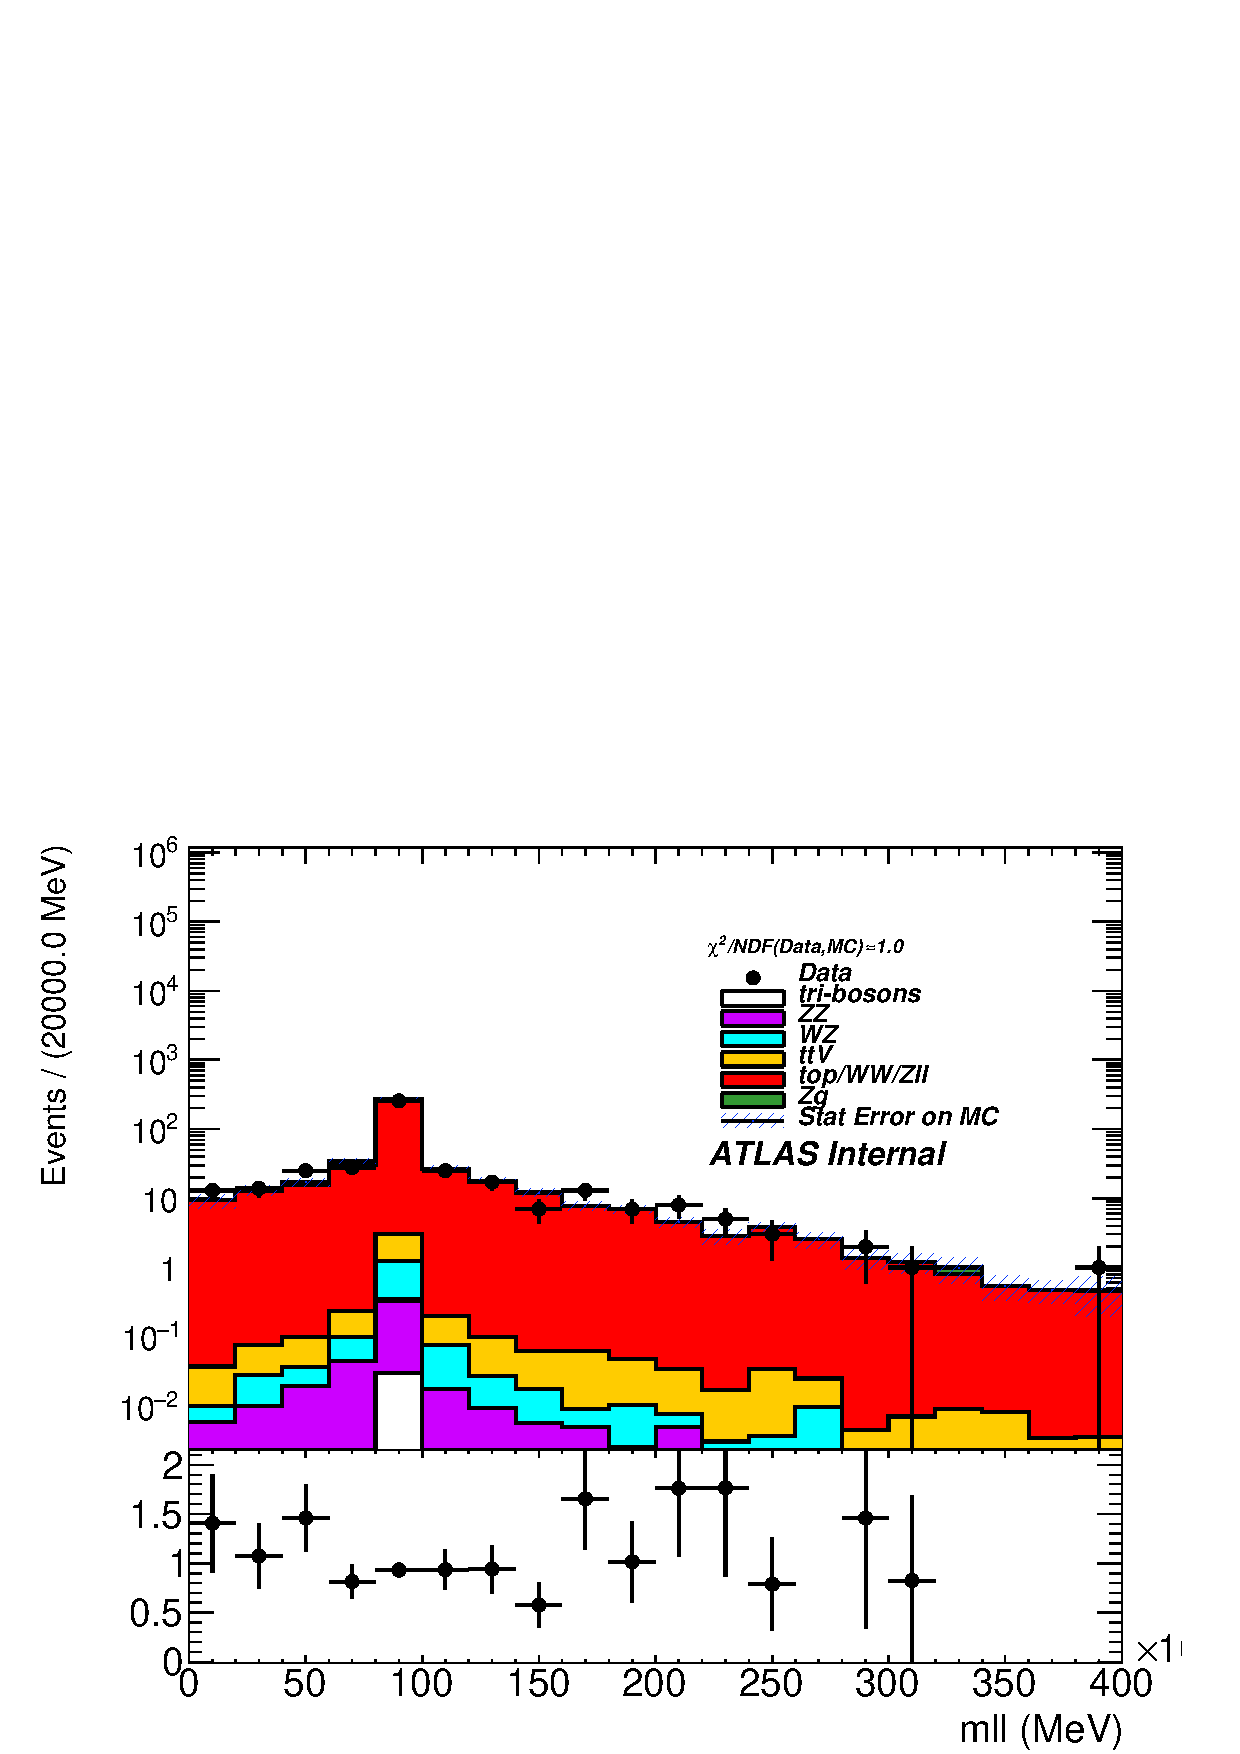
\includegraphics[width=0.45\textwidth]{figures/WZ_CR/2DSideband_WZCR_NonIsolated}
\caption{ Distribution of $m_{\ell\ell}^{SFOS}$ in the isolated and  non-isolated 
control regions. The agreement between the data and the MC expectation
is not expected to be perfect, since the MC does not do a good job 
of modeling the fake background. The 2D sideband method uses the data
to estimate the fake background.}
\label{fig:wz_sidebands}
\end{figure}

If we can solve the equations above for $N^{WZ}_{A,B}$ in the signal region
(when $A=\textrm{With \z-veto}$ and $B=\textrm{Isolated}$)
then we have our estimate. 
This is 5 equations and 16 unnkowns. The four unknowns, $N^{\textrm{Data}}_{A,B}$,
are determined using the data directly while 
the electroweak backgrounds, $N^{\textrm{Electroweak}}_{A,B}$,
and the $WZ$ contributions in the sidebands, $N^{WZ}_{A,B}$ 
(when $A=\textrm{With \z-veto}$ and $B=\textrm{Isolated}$ are not both true)
are determined using $WZ$ MC. This reduces the problem to 5 equations
and 5 unknowns and so we can solve algebraically for the remaining unkowns
including the desired value for the $WZ$ estimate in the signal region.

\begin{table}
\centering


\begin{tabular}{|cc|cc|}
\hline
%\multicolumn{3}{|c|}{$N^{\textrm{Data}}_{A,B}$}\\
\multirow{3}{*}{$N^{\textrm{Data}}_{A,B}$}&
\backslashbox{A}{B}& Isolated & Non-Isolated \\
\cline{2-4}
&With \z-veto & $724\pm27$ & $272\pm16$ \\
&Without \z-veto & $67\pm8$  & $118\pm11$ \\
\hline
\hline
%\multicolumn{3}{|c|}{$N^{\textrm{Electroweak}}_{A,B}$}\\
\multirow{3}{*}{$N^{\textrm{Electroweak}}_{A,B}$}&
\backslashbox{A}{B}& Isolated & Non-Isolated \\
\cline{2-4}
&With \z-veto & $172\pm3$ & $7.7\pm0.9$ \\
&Without \z-veto & $29\pm2$  & $1.9\pm0.6$ \\
\hline\hline
%\multicolumn{3}{|c|}{$N^{WZ}_{A,B}$ (MC)}\\
\multirow{3}{*}{$N^{WZ}_{A,B}$}&
\backslashbox{A}{B}& Isolated & Non-Isolated \\
\cline{2-4}
%&With \z-veto & $498\pm1$& $0.896\pm0.050$ \\
&With \z-veto & ---& $0.896\pm0.050$ \\
&Without \z-veto & $31.82\pm0.35$  & $0.095\pm0.015$ \\
\hline
\end{tabular}

\caption{All of the inputs used to constrain the system of five equations
from \eqn\eqref{eq:wzparam} and \eqn\eqref{eq:wz_constraint}.
The values are derived in the signal region and three sideband regions
described in the text. $N^{\textrm{Data}}_{A,B}$ are determined directly
from the data; $N^{\textrm{Electroweak}}_{A,B}$ and $N^{WZ}_{A,B}$ are 
determined in MC. The value for $N^{WZ}_{\textrm{With \z-veto,Isolated}}$ is
not used as an input and is instead solved for as the the main
parameter of interest. Still, the value is determined in MC to be
$498 \pm 1$.  Only statistical uncertainties are shown.}
\label{tab:wz_input}
\end{table}

\begin{table}
\centering


\begin{tabular}{|cc|cc|}
\hline
%\multicolumn{3}{|c|}{$N^{\textrm{Data}}_{A,B}$}\\
\multirow{3}{*}{$N^{\textrm{Fake}}_{A,B}$}&
\backslashbox{A}{B}& Isolated & Non-Isolated \\
\cline{2-4}
%&With \z-veto & $8\pm23$ &  \\ %this is the number provided by louis
&With \z& $14 \pm 43$ & $263\pm 16 $\\
&Without \z&  $6.2 \pm 8.3$ & $116 \pm 11$\\
\hline
\hline
\multirow{3}{*}{$N^{WZ}_{A,B}$}&
\backslashbox{A}{B}& Isolated & Non-Isolated \\
\cline{2-4}
&With \z& $537\pm35$ & --- \\ %I calculated 537.97 \pm 33.04
&Without \z& ---  & --- \\
\hline
\end{tabular}

\caption{Outputs from the system of five equations
from \eqn\eqref{eq:wzparam} and \eqn\eqref{eq:wz_constraint}
after including the numbers from \tab\ref{tab:wz_input} as input.
The value for $N^{WZ}_{\textrm{With \z-veto, Isolated}}$ is 
the value of primary interest.  Only statistical uncertainties are shown.}
\label{tab:wz_output}
\end{table}


The inputs to the system of equations are summarized in 
\tab\ref{tab:wz_input}\footnote{Note that the $WZ$ MC prediction in 
the signal region is not used expect as a comparison.}.
The derived values after solving the system of equations are
summarized in \tab\ref{tab:wz_output}. 
The derived estiamte for the $WZ$ contribution to 
the signal region is 
$537 \pm 35$
events, where the uncertainty is purely statistical. 
Compare this to the estimate from MC of 
$498 \pm 1$ events.
The ratio of the two can be used to derive a k-factor of
$1.08\pm0.07\stat$.


Systematic uncertainties are also derived on the method
by varying the 
thresholds used to define the sideband regions, varying the normalization
of the MC estimates in \tab\ref{tab:wz_input}, and by varying the degree
of equality in \eqn\eqref{eq:wz_constraint}. The effect of each
uncertainty is propogated to the estimate of the $WZ$ normalization in
the signal region and are combined in quadrature. The total systematic
uncertainty is found to be 5.9\%. 
The final k-factor is thus $1.08 \pm0.07\stat\pm0.07\syst$.

The derived k-factor is applied to the MC estimate in another control
region enhanced in the $WZ$ process. This control region is determined
using the pre-selection region as described in \sec\ref{sec:preselection}
plus an additional requirement that there be 2 SFOS lepton pairs.
This gives a good test of the $WZ$ normalization in a control region
which is closer to the $WWW$ signal regions. 
This comparison is shown in \fig\ref{fig:WZ_2SFOS_CR}. 
The data is shown to be in good agreement with the corrected $WZ$ MC
estimate as desired.

\begin{figure}[htp]
\centering
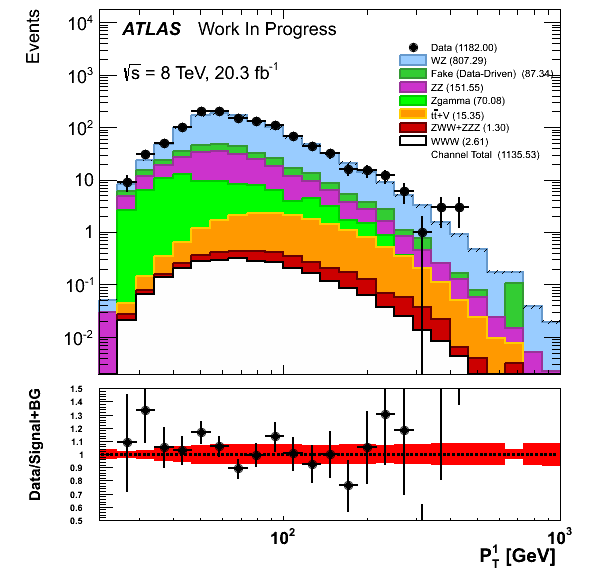
\includegraphics[width=0.4\textwidth]{figures/WZ_CR/LeadingLeptonPt_histratio.png}
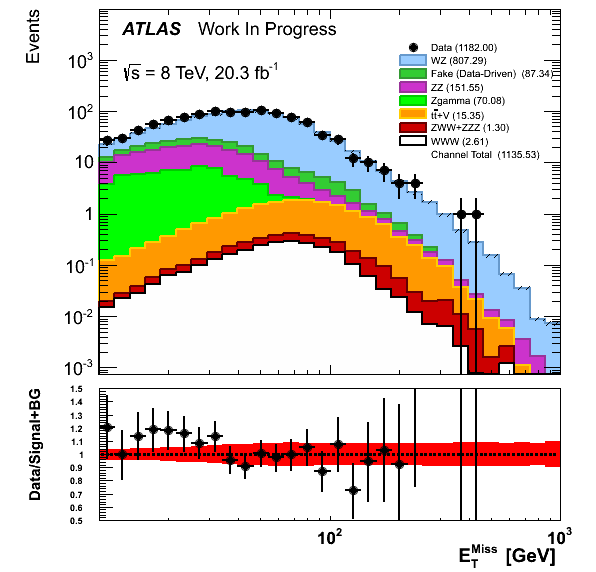
\includegraphics[width=0.4\textwidth]{figures/WZ_CR/MET_Et_histratio.png}
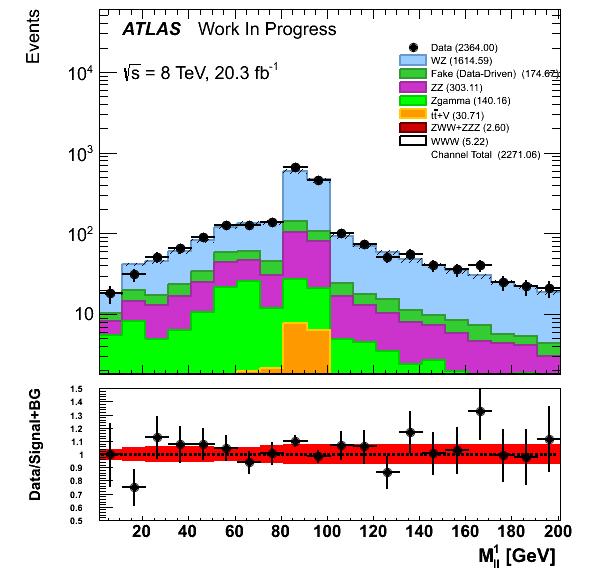
\includegraphics[width=0.4\textwidth]{figures/WZ_CR/InvariantMassSFOS_histratio.png}
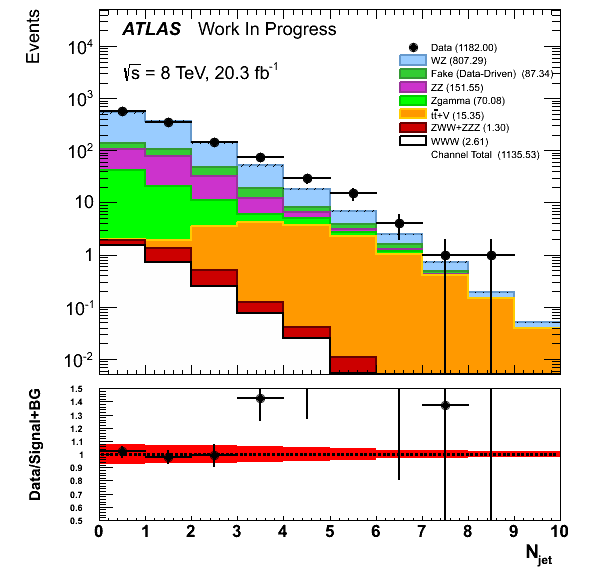
\includegraphics[width=0.4\textwidth]{figures/WZ_CR/NJets_histratio.png}
\caption{$WZ$ 2SFOS Control regions. Distribution of leading lepton $p_{T}$, $\MET$, $m_{12}$, and jet multiplicity. The systematic band shows the uncertainty on the WZ k-factor.}
\label{fig:WZ_2SFOS_CR}
\end{figure}  

As a further test of the method, a MC estimate which includes the $WZ$ signal as
well as the Electroweak and fake backgrounds is used as input in place 
of $N^{\textrm{Data}}_{A,B}$ to see if the the MC estimate for the $WZ$
contribution in the signal region can be recovered. This is referred to as
a closure test.  The measured value for the $WZ$ normalization from the 
closure test is found to be  $495\pm39$, which is indeed consistent with the
estimate from pure MC of $498\pm1$. The closure test also shows consistent
results when varying the normalizations of the different compoenents 
in the MC independently.




\subsubsection{$ZZ\rightarrow llll$}
\label{sec:zzbg}

The $ZZ\rightarrow llll$ process has a similar cross-section as 
the $WZ\rightarrow lll\nu$ process but is 
suppressed by the probability that exactly one lepton is not reconstructed. 
Still, this probability is large enough this is one of the largest backgrounds
in the 1 and 2 SFOS signal regions. These are simulated
using MC as descrbed in \sec\ref{sec:www_bg_samples}.
Unlike the $WZ$ process, NNLO predictions are available 
from~\cite{Cascioli:2014yka,Baglio:2013toa,Bierweiler:2013dja}
that suggest a k-factor of 1.05 on the overall $ZZ$ prediction.
The uncertainty on the prediction is determined to be 
15\%~\cite{Cascioli:2014yka,Baglio:2013toa,Bierweiler:2013dja}.
This correction is used instead of determining a correction in the data
as was performed for the $WZ$ process in \sec\ref{sec:wzbg}.
STOP


The agreement between data and the model is then checked in a control region, where 2 same flavors opposite sign pairs leptons ($e$ and $\mu$) are requested. The leptons must follow the quality requirements defined in Section~\ref{sec:Object_selection}. The transverse momentum of the leptons should be: $p_{T}^{1}>25~\GeV$, $p_{T}^{2}>15~\GeV$, $p_{T}^{3}>15~\GeV$, and  $p_{T}^{4}>10~\GeV$. The pairing of the leptons follows the algorithm defined in~\cite{Aad:2014wra}. In order to remove any contribution from fake backgrounds, only the events where the two $Z$ bosons are on shell are kept, \textit{ie}: $60<m_{12}<120~\GeV$ and $60<m_{34}<120~\GeV$. Figure~\ref{fig:ZZ_CR}, show the distributions of $m_{12}$, $m_{34}$, $m_{4l}$, and the leptons $p_{T}$ for this selection, while Table~\ref{tab:ZZ_CR} gives the total number of event measured in this CR and the prediction on the different processes in the same region.

The agreement between the data and the MC predictions is very good, for the shape or for the prediction of the total number of events in this control region.

It was also checked whether or not the contribution of $ZZ^{*}$ where the $Z^{*}$ boson is very offshell, $m_{Z^{*}} < 4$~GeV, while the other boson
has a  mass $m_Z > 4$~GeV has any impact on the signal regions. This was evaluted by looking at the samples with channel numbers
$181471$ through $181479$ in Table~\ref{tab:sample_bkg_dibosons}.  The contribution from these samples were found to be negligible, with a statistical
uncertainty compatible with exaxtly 0 events in the individual signal regions. As a result, these samples were not considered any further and are not
included in the final background  estimate for the signal regions or in the ZZ control regions.


\begin{figure}[htp]
\centering
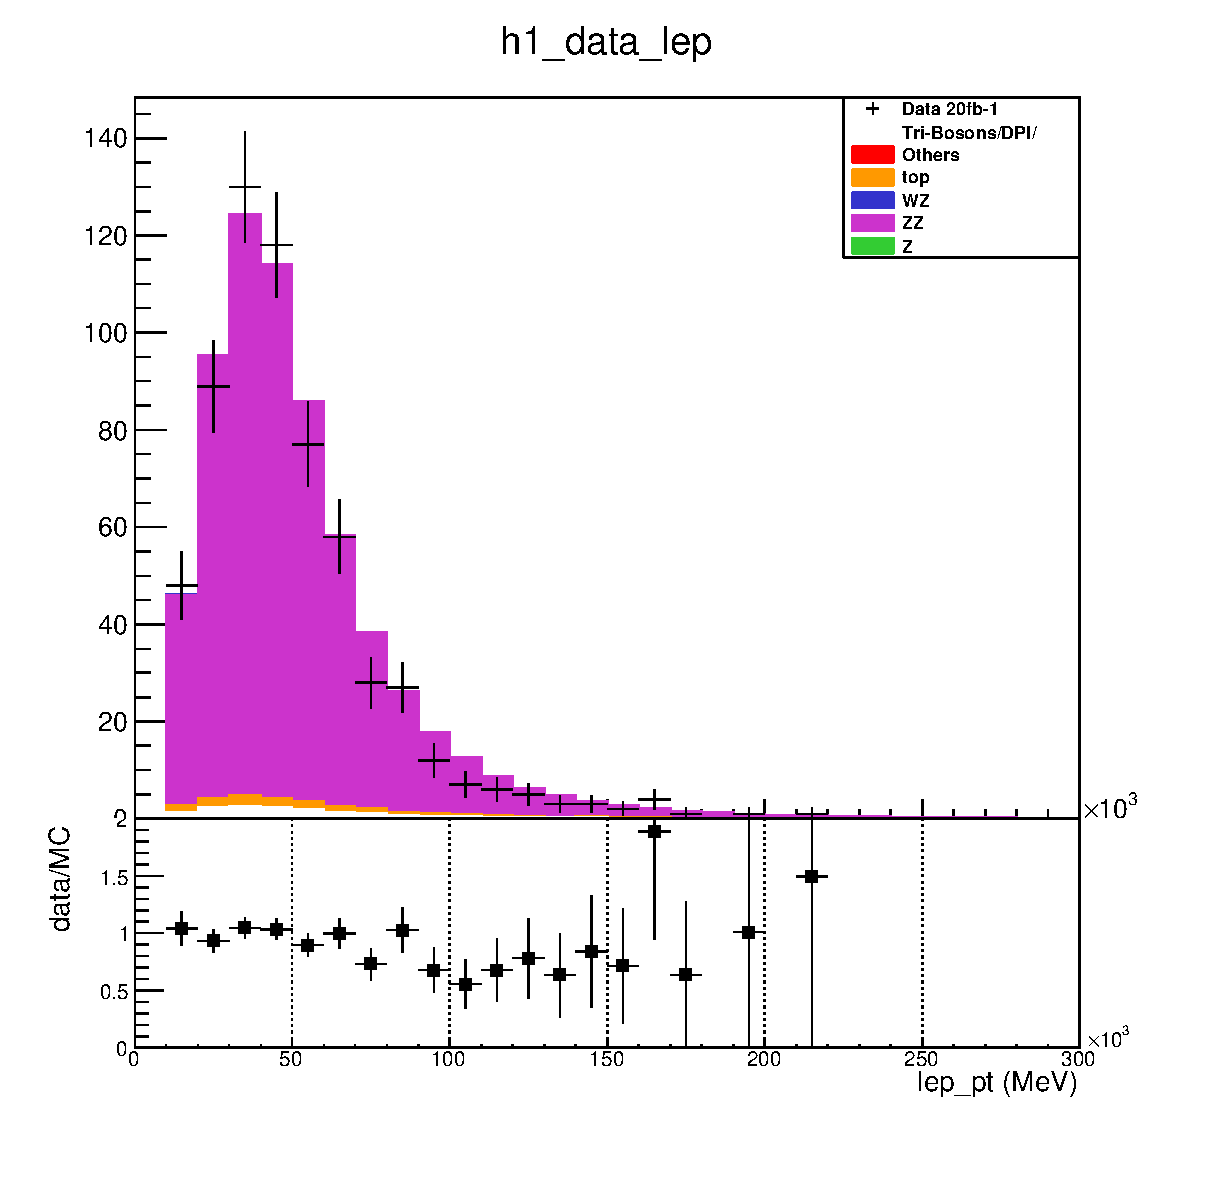
\includegraphics[width=0.4\textwidth]{figures/ZZ_CR/ZZ_CR_lep_pt.eps}
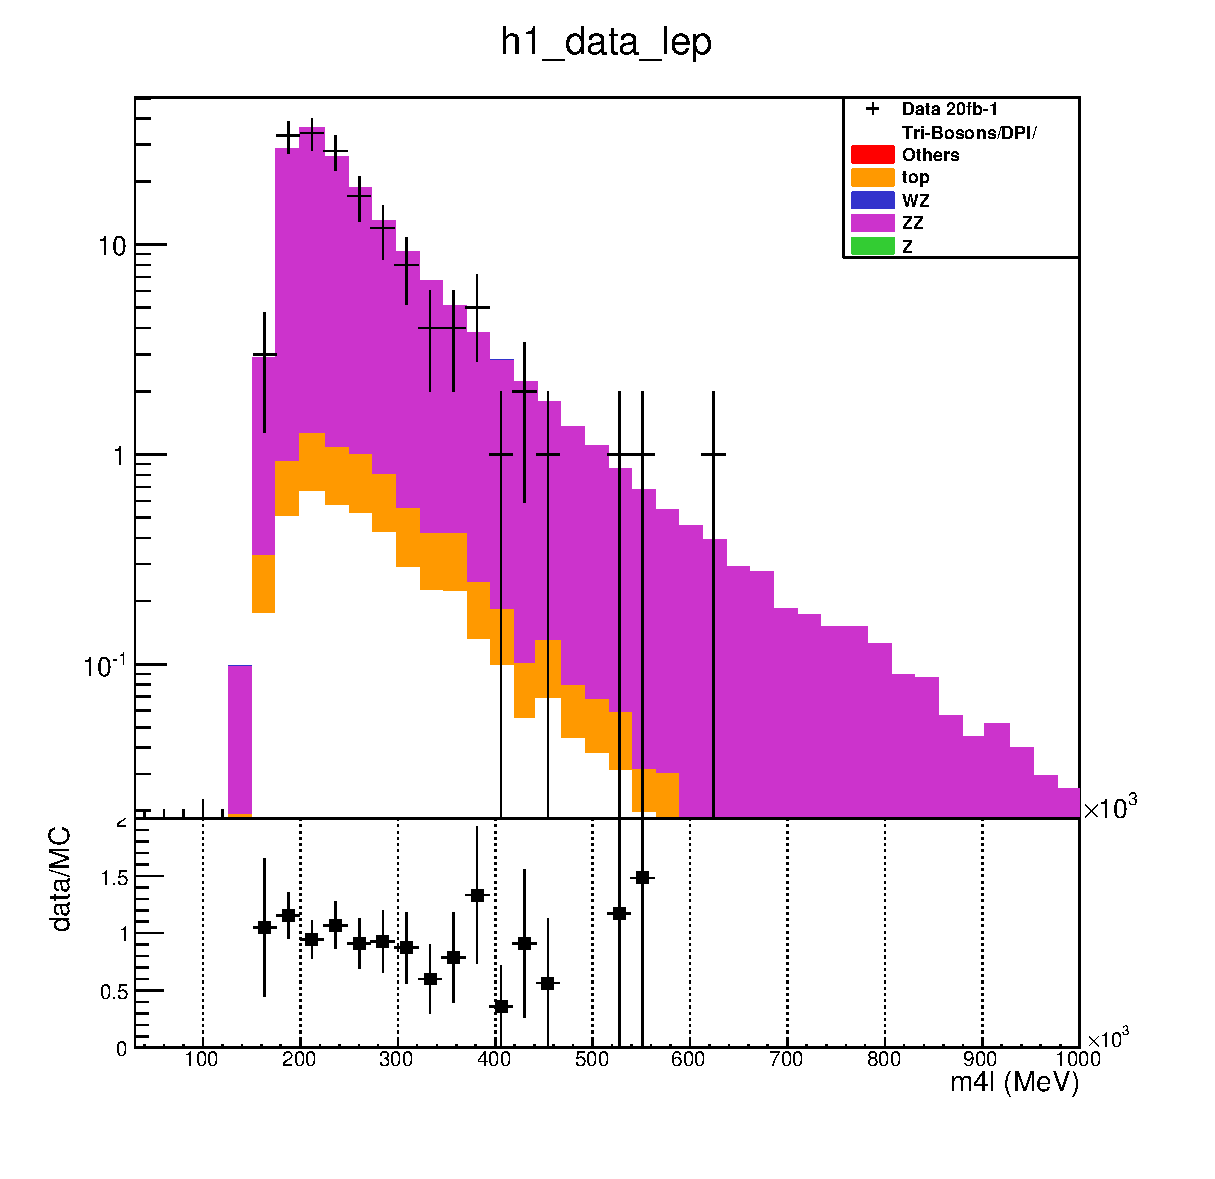
\includegraphics[width=0.4\textwidth]{figures/ZZ_CR/ZZ_CR_m4l.eps}
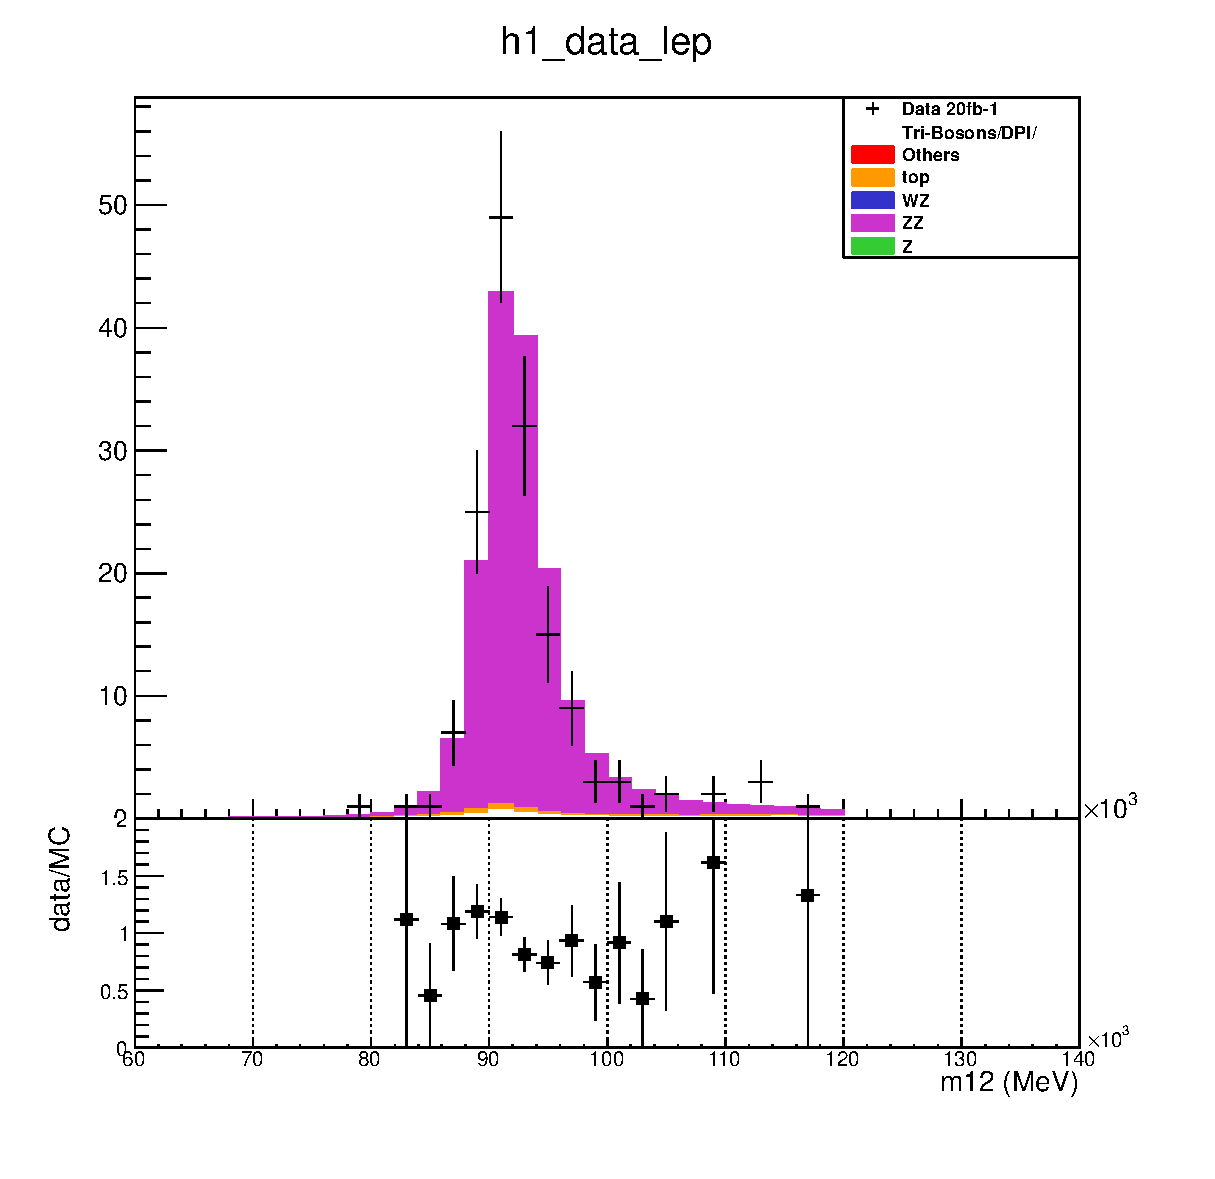
\includegraphics[width=0.4\textwidth]{figures/ZZ_CR/ZZ_CR_m12.eps}
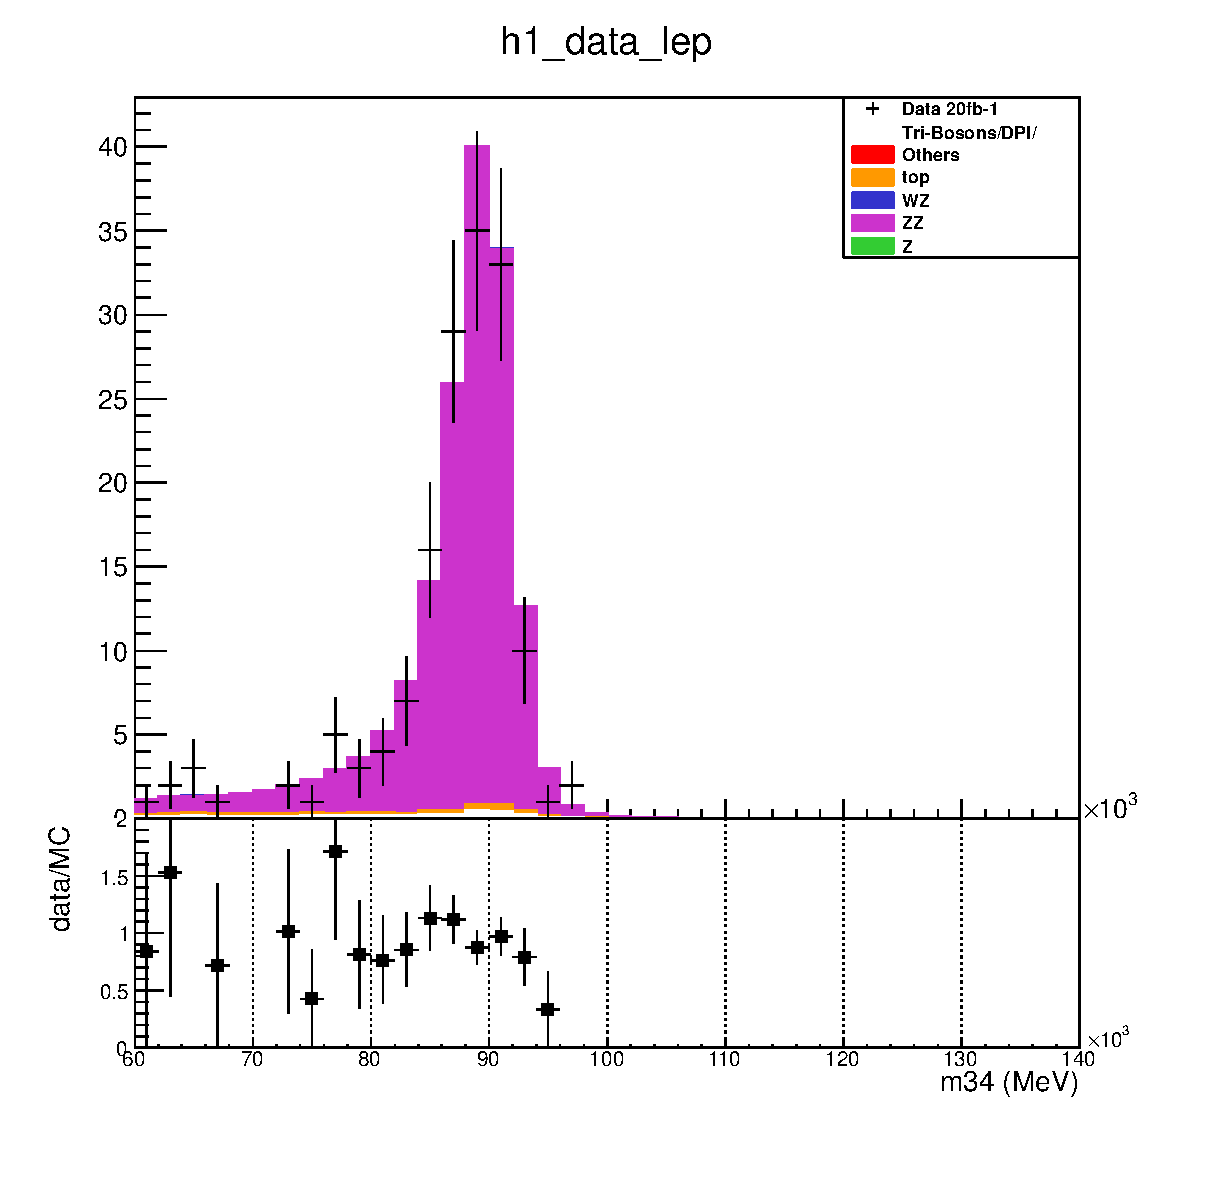
\includegraphics[width=0.4\textwidth]{figures/ZZ_CR/ZZ_CR_m34.eps}

\caption{$ZZ\to{}4\ell$ Control regions. Distribution of leptons $p_{T}$, $m_{12}$, $m_{34}$, $m_{4l}$.}
\label{fig:ZZ_CR}
\end{figure}  

\begin{table}[htp]
\centering
\begin{tabular}{|c||c|c|c|c|}
\hline
 & Event Yield\\ 
\hline\hline
$WZ$ &  $0.05 \pm 0.01$\\ 
$ZZ$ &  $156.2 \pm 0.3$(stat) $\pm 22.3$(syst) \\ 
% $gg2ZZ$ &	$21.3 \pm 0.2$ \\
$Z\gamma$ &  $0.0 \pm 0.0$\\ 
Fake (MC) &  $3.6 \pm 0.2$\\ 
triboson and $t\bar{t}+V$ &  $4.1 \pm 0.2$\\ 
\hline
Expected Signal + Background &  $164.0 \pm 0.3$ (stat) $\pm 22.3$(syst)\\ 
\hline
Observed Data &  $155 \pm 12$\\ 
\hline
\end{tabular}
\caption{Number of data and predicted events in the ZZ CR. The error quoted on the MC samples represents only the statistical error on the MC samples. The systematic error due to theoretical normalization on the $ZZ$ sample is also showed.}
\label{tab:ZZ_CR}
\end{table}


\clearpage

\subsubsection{$Z\gamma$}

The $Z\gamma$ process, where the $Z$ boson decays to a pair of leptons ($e$ and $\mu$), is estimated from MC. This proces is obtained using the Sherpa generator. It was found that Sherpa describes accurately the shape and normalization of data in the $7~\TeV$ and $8~\TeV$ datasets~\cite{Aad:2013izg,Auerbach:1631102}. Therefore the normalization of these sample is taken to be the cross-section provided by the Sherpa generator. These processes are contributing to our selection, via the conversion of one photon into a pair of electrons, and then the loss of one of these electrons in the acceptance. 

These effects are expected to be properly described by the simulation, but the agreement between the data and the model is checked in a control region where the events are requested to contains exactly two muons and one electron, and the tri-body invariant mass of this system, should be close to the $Z$-pole mass~\cite{PDG:2014}: $|m_{\mu\mu{}e}-91.19|<15~\GeV$.

Figure~\ref{fig:Zgamma_CR} shows the invariant mass distribution of the 3 leptons, the leptons $p_{T}$, the $\eta$ distribution of the electron, and the jet multiplicity. The normalization in the CR is also checked and is provided in Table~\ref{tab:Zgamma_CR}.
All the distributions and the event yield show a very good agreement between the data and the model.

\begin{figure}[htp]
\centering
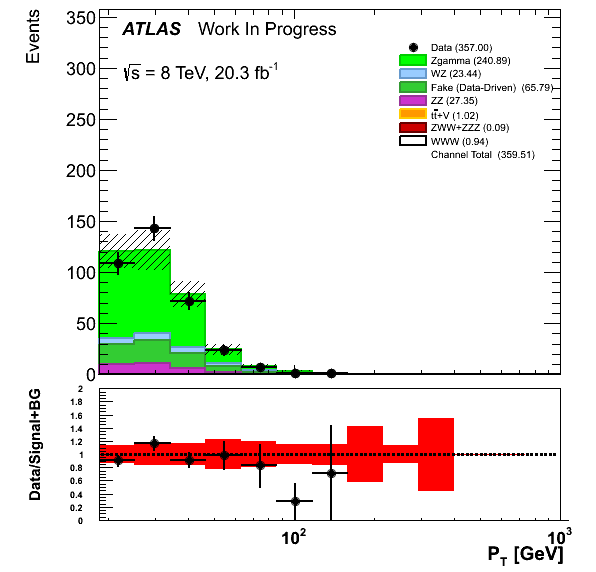
\includegraphics[width=0.4\textwidth]{figures/ZG_CR/AllLeptonPt_histratio.png}
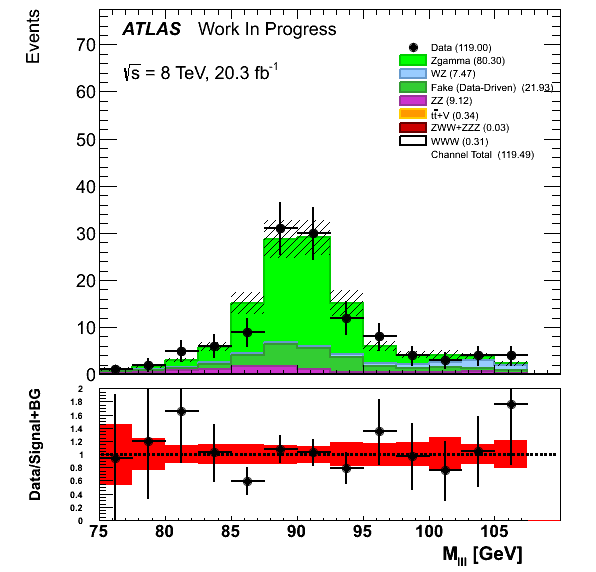
\includegraphics[width=0.4\textwidth]{figures/ZG_CR/InvariantMassThreeLep_histratio.png}
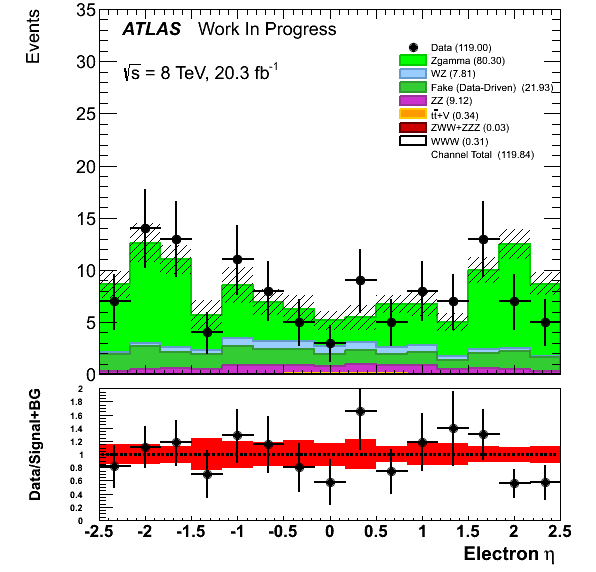
\includegraphics[width=0.4\textwidth]{figures/ZG_CR/ElectronEta_histratio.png}
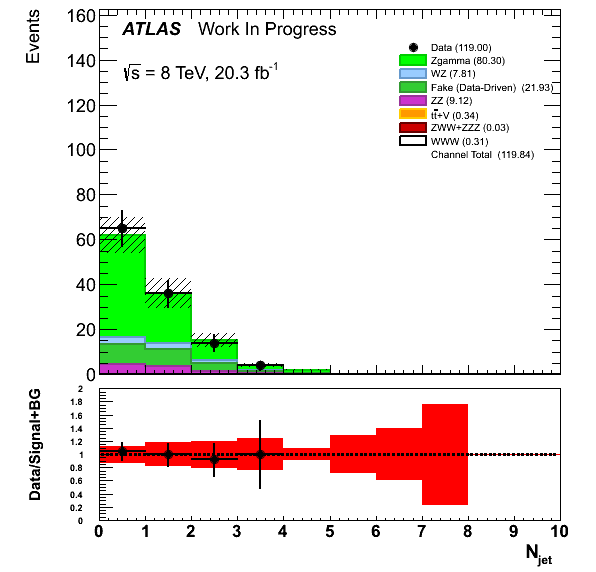
\includegraphics[width=0.4\textwidth]{figures/ZG_CR/NJets_histratio.png}

\caption{$Z\gamma$ Control region. Distribution of leptons $p_{T}$, invariant mass of the 3leptons, electron $\eta$, and jet multiplicity.}
\label{fig:Zgamma_CR}
\end{figure}  


\begin{table}[ht!]
\centering
\begin{tabular}{|c||c|c|c|c|}
\hline
 & Event Yield\\ 
\hline\hline
$WZ$ &  $7.47 \pm 0.11$\\ 
$ZZ$ &  $9.116 \pm 0.075$\\ 
$Z\gamma$ &  $80.3 \pm 2.8$\\ 
$ZWW+ZZZ$ &  $0.0285 \pm 0.0046$\\ 
$t\bar{t}+V$ &  $0.338 \pm 0.012$\\ 
Fake (data-driven) &  $21.9 \pm 1.2$\\ 
$WWW$ &  $0.3142 \pm 0.0072$\\ 
\hline
Expected Background &  $119.2 \pm 3.1$\\ 
Expected Signal + Background &  $119.5 \pm 3.1$\\ 
\hline
Observed Data &  $119 \pm 11$\\ 
\hline
\end{tabular}

\caption{Expected and observed event yields for the Z$\gamma$ control region. Only the statistical uncertainties are showed.}
\label{tab:Zgamma_CR}
\end{table}



\subsubsection{Double parton scattering, $\ttbar + V$, and $VVV$}

\paragraph{DPS}
\label{sec:bkg_DPS}
Double parton scattering (DPS) backgrounds are also taken into account in the analysis. To estimate their contribution a list of samples used in the same sign WW analysis~\cite{Aad:2014zda,DPS:Twiki} has been used. The cross section of these processes can not be taken directly from MC, but it must be further studied. Considering the DPS production of $A+B$, where $A$ and $B$ can be products of any single-parton, the cross section can can be factorised as~\cite{Gaunt:2010pi}:
\begin{equation}
	\sigma^{DPS}_{(A+B)}=\frac{m}{2}\times{}\frac{\sigma^{S}_{A}\times{}\sigma^{S}_{B}}{\sigma_{eff}}
\end{equation}	

Where $\sigma^{S}_{(A/B)}$ is the single-parton scattering production cross-section of the process $A/B$, $m$ is a factor which takes the value of 1 when $A=B$ and 2 when $A\ne B$, $\sigma_{eff}$ is the effective cross section of the proton. A measurement of $\sigma_{eff} =15\pm3(stat)^{+5}_{-3}(syst)$ mb for 7~\TeV{} $p-p$ collisions has been recently performed by ATLAS~\cite{Aad:2013bjm}. By factorizing the cross-section in this form, the correlation between the two parton interactions are neglected.

The samples and cross section that have been used in this analysis are given in Table~\ref{tab:sample_bkg_dibosons_gg2DPI}. An uncertainty of $50\%$ is applied on the normalization of these processes. Among these processes the one that can give a tri-lepton final state are: $WZ$, $ZZ$, and $Z\gamma$.
	
Their contributions are found to be negligible.


\paragraph{Other backgrounds}
The other backgrounds evaluated from MC are the one containing three real leptons: $t\bar{t}+V$, $WWZ$, and $WZZ$.
The PDF and scale uncertainties for the $t\bar{t}+V$ processes have been evaluated by other member of the ATLAS collaboration~\cite{ttV:Twiki}, and found
to be about $30\%$ of their normalization. These processes have been recently measured by the ATLAS collaboration~\cite{ATLAS-CONF-2015-032}, and their normalization are found to be consistent with the NLO predictions.

An equivalent $30\%$ uncertainty is assigned for the other $VVV$ contributions ($ZWW^{*}$ and $ZZZ^{*}$) that are not coming from our signal.

% Other background contributions are arising from tt¯+V, t+V and VVV processes. They will be estimated
%  using MC samples and global normalization uncertainties are associated to these MC predictions. An
%  uncertainty of 30\% is assigned to the tt¯+ V contribution, according to [27]. An uncertainty of 30\% is
%  also assigned to the VVV contribution.
